%%
	%Latent Factor Model Repetition
	%Created by Vulcan626 on 2023.9.20	
%%
\documentclass{beamer}
\usepackage{graphicx}
\usepackage{amsmath}
\usepackage{cite} % For citations
\usepackage{hyperref} % For clickable links in the references
\usepackage[absolute,overlay]{textpos}
\usepackage{tikz}
\usepackage[UTF8]{ctex}
\usepackage{tabularx}

%代码设置
\usepackage{fancybox}
\usepackage{xcolor}
\usepackage{times}
\usepackage{listings}

\definecolor{mygreen}{rgb}{0,0.6,0}
\definecolor{mygray}{rgb}{0.5,0.5,0.5}
\definecolor{mymauve}{rgb}{0.58,0,0.82}
\newcommand{\Console}{Console}
\lstset{ %
	backgroundcolor=\color{white},   % choose the background color
	basicstyle=\footnotesize\rmfamily,     % size of fonts used for the code
	columns=fullflexible,
	breaklines=true,                 % automatic line breaking only at whitespace
	captionpos=b,                    % sets the caption-position to bottom
	tabsize=4,
	commentstyle=\color{mygreen},    % comment style
	escapeinside={\%*}{*)},          % if you want to add LaTeX within your code
	keywordstyle=\color{blue},       % keyword style
	stringstyle=\color{mymauve}\ttfamily,     % string literal style
	numbers=left, 
	%frame=single,
	rulesepcolor=\color{red!20!green!20!blue!20},
	%identifierstyle=\color{red},
	language=c
}

\mode<presentation>
{
\usetheme{Madrid}
\usecolortheme{default}
}

%Change the reference icon to a standard format
\setbeamertemplate{bibliography item}[text]

%------TITLE PAGE------
\title[LFM]{隐语义模型复现}
%\subtitle{Transforming Insights through Data Science on Big Data Platforms}
\author[Authors]{华展博 \and 王知秋 \and 张昊坡 \and 张晓佩}
\institute[CUMT]{计算机科学与技术学院 \\ 中国矿业大学}
\date{2023年9月21日}

\iffalse
%------Highlight the title of the current section------
\AtBeginSection[]
{
	\begin{frame}
		\frametitle{Table of Contents}
		\tableofcontents[currentsection]
	\end{frame}
}
\fi


\begin{document}

% Logo at the top center
\begin{textblock*}{5cm}(5.7cm,0.1cm) % Adjust the position as needed

\includegraphics[width=1.5cm]{fig/logo0.png}
\end{textblock*}

%insert title page
\frame{\titlepage}

\makeatletter
\setbeamertemplate{footline}{
  \ifnum\c@framenumber>1%
    \tikz[remember picture,overlay]{
      \node at (current page.north east) [anchor=north east, yshift=-0.2cm] {
\includegraphics[width=5cm]{fig/logo1.png}};
    }
  \fi
}
\makeatother

%insert contents
\begin{frame}
	\frametitle{目录}
	\tableofcontents
\end{frame}

%Introduction
\section{介绍}
	%Frame0
	\begin{frame}
	\frametitle{介绍}
		\begin{itemize}
  			\item 隐语义模型是最近几年推荐系统领域最为热门的研究话题,它的核心思想是通过隐含特征(latent factor)联系用户兴趣的物品
  			\item 为了从数据角度出发准确的给物品分类然后进行个性化推荐,隐含语义分析技术采取基于用户行为统计的自动聚类,较好的解决了相关问题。
  			\item 我们将以LFM为例,使用Movielens ml-1m数据集分析其在推荐系统的应用。
		\end{itemize}
	\end{frame}

%The underlying algorithm
\section{基础算法}
	%Frame0
	\begin{frame}{基础算法}
			\lstinputlisting[lastline=6,
							language=Python,
							frame=single,
							caption=Import the package,
							label=python]
							{py/0.py}
	\end{frame}
	%Frame1
	\begin{frame}{基础算法}
			\lstinputlisting[lastline=9,
							language=Python,
							frame=single,
							caption=Generic function definitions,
							label=python]
							{py/1.py}
	\end{frame}
	%Frame2
	\begin{frame}{基础算法}
			\lstinputlisting[lastline=12,
							language=Python,
							frame=single,
							caption=LoadData,
							label=python]
							{py/2.py}
	\end{frame}
	%Frame3
	\begin{frame}{基础算法}
			\lstinputlisting[lastline=17,
							language=Python,
							frame=single,
							caption=SplitData,
							label=python]
							{py/3.py}
	\end{frame}
	%Frame4
	\begin{frame}{基础算法}
			\lstinputlisting[lastline=11,
							language=Python,
							frame=single,
							caption=Convert dict,
							label=python]
							{py/4.py}
	\end{frame}
	%Frame5
	\begin{frame}{基础算法}
			\lstinputlisting[lastline=16,
							language=Python,
							frame=single,
							caption=Metric,
							label=python]
							{py/5.py}
	\end{frame}
	%Frame6
	\begin{frame}{基础算法}
			\lstinputlisting[lastline=20,
							language=Python,
							frame=single,
							caption=Metric,
							label=python]
							{py/6.py}
	\end{frame}
	%Frame7
	\begin{frame}{基础算法}
			\lstinputlisting[lastline=18,
							language=Python,
							frame=single,
							caption=LFM,
							label=python]
							{py/7.py}
	\end{frame}
	%Frame8
	\begin{frame}{基础算法}
			\lstinputlisting[lastline=18,
							language=Python,
							frame=single,
							caption=LFM,
							label=python]
							{py/8.py}
	\end{frame}
	%Frame9
	\begin{frame}{基础算法}
			\lstinputlisting[lastline=18,
							language=Python,
							frame=single,
							caption=LFM,
							label=python]
							{py/9.py}
	\end{frame}
	%Frame10
	\begin{frame}{基础算法}
			\lstinputlisting[lastline=19,
							language=Python,
							frame=single,
							caption=Experiment,
							label=python]
							{py/10.py}
	\end{frame}
	%Frame11
	\begin{frame}{基础算法}
			\lstinputlisting[lastline=19,
							language=Python,
							frame=single,
							caption=Experiment,
							label=python]
							{py/11.py}
	\end{frame}
	%Frame12
	\begin{frame}{基础算法}
			\lstinputlisting[lastline=19,
							language=Python,
							frame=single,
							caption=Experiment,
							label=python]
							{py/12.py}
	\end{frame}
	%FrameTable1
	\begin{frame}{基础算法}
	\framesubtitle{LFM性能(ratio=1)}
		\begin{table}[h]
		\centering
		\caption{实验结果(比例=1)}
			\begin{tabular}{|c|c|c|c|c|}
			\hline
			实验编号 & 精度 & 召回率 & 覆盖率 & 流行度 \\
			\hline
			0 & 19.15\% & 9.2\% & 88.35\% & 6.3121 \\
			1 & 19.01\% & 9.1\% & 87.85\% & 6.3099 \\
			2 & 19.06\% & 9.11\% & 87.71\% & 6.3076 \\
			3 & 18.92\% & 9.09\% & 88.81\% & 6.3017 \\
			4 & 18.9\% & 9.09\% & 88.3\% & 6.3162 \\
			5 & 18.96\% & 9.15\% & 88.24\% & 6.3114 \\
			6 & 18.7\% & 8.99\% & 88.78\% & 6.3055 \\
			7 & 18.69\% & 8.96\% & 88.3\% & 6.2934 \\
			\hline
			\multicolumn{5}{c}{平均结果 (M=8, N=10, 比例=1)} \\
			\hline
 			ratio=1 & 18.92\% & 9.09\% & 88.29\% & 6.3072 \\
			\hline
			\end{tabular}
		\end{table}
	\end{frame}
	%FrameTable2
	\begin{frame}{基础算法}
	\framesubtitle{LFM性能(ratio=2)}
		\begin{table}[h]
		\centering
		\caption{实验结果(比例=2)}
			\begin{tabular}{|c|c|c|c|c|}
			\hline
			实验编号 & 精度 & 召回率 & 覆盖率 & 流行度 \\
			\hline
			0 & 22.95\% & 11.02\% & 40.81\% & 6.9484 \\
			1 & 23.09\% & 11.06\% & 40.81\% & 6.9389 \\
			2 & 23.24\% & 11.11\% & 41.06\% & 6.9401 \\
			3 & 22.86\% & 10.99\% & 40.57\% & 6.9447 \\
			4 & 22.77\% & 10.95\% & 41.02\% & 6.9419 \\
			5 & 22.82\% & 11.00\% & 40.4\% & 6.9468 \\
			6 & 22.78\% & 10.95\% & 40.81\% & 6.9465 \\
			7 & 22.80\% & 10.93\% & 41.18\% & 6.9406 \\
			\hline
			\multicolumn{5}{c}{平均结果 (M=8, N=10, 比例=2)} \\
			\hline
 			ratio=2 & 22.91\% & 11.00\% & 40.83\% & 6.9435 \\
			\hline
			\end{tabular}
		\end{table}
	\end{frame}
	%FrameConclusion
	\begin{frame}
	\frametitle{{基础算法}}
	\framesubtitle{LFM性能}
		\begin{columns}
			\begin{column}{0.5\textwidth}
				\begin{itemize}
					\item 随着负样本数目的增加,LFM的准确率和召回率有明显提高。
					\item 覆盖率相对较高,说明数据集中的大部分物品都得到了推荐。
					\item 流行度指标表明推荐的物品不会过于热门,这对于推荐多样性来说是一个积极的迹象。
					\item 当ratio>10以后,准确率和召回率基本稳定在25\%和13\% 。
				\end{itemize}
			\end{column}
			\begin{column}{0.5\textwidth}
				\begin{figure}
        		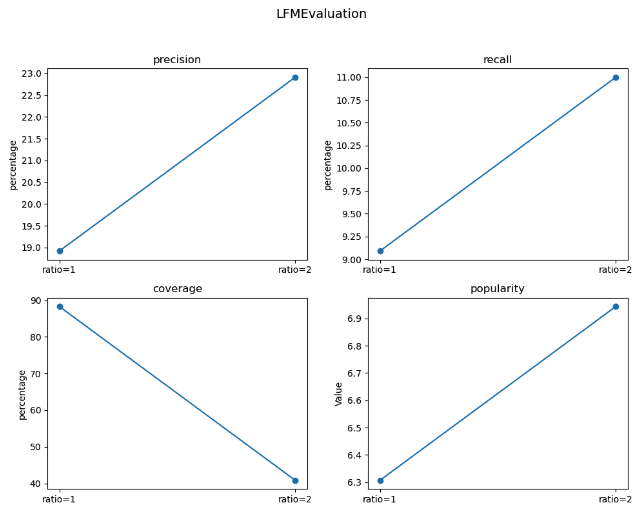
\includegraphics[width=\linewidth]{fig/myplot.png} % Adjust the path and size of the image
        		\caption{LFM Evaluation}
      			\end{figure}
			\end{column}
		\end{columns}
	\end{frame}
%Algorithm optimization
\section{算法优化}
	%Frame0
	\begin{frame}
	\frametitle{算法优化}
	\framesubtitle{加入偏置(Bias)部分}
		\begin{itemize}
  			\item 我们观测到的评分数据大部分都是都是和用户或物品无关的因素产生的效果,即有很大一部分因素是和用户对物品的喜好无关而只取决于用户或物品本身特性的。
  			\item 这些独立于用户或独立于物品的因素称之为偏置(Bias)部分。
  			\item 在矩阵分解模型中偏置部分对提高评分预测准确率起的作用要大大高于个性化部分所起的作用。
		\end{itemize}
	\end{frame}
	%Frame1
	\begin{frame}
	\frametitle{算法优化}
	\framesubtitle{加入偏置(Bias)部分}
		\textbf{目标函数}\\
		偏置部分主要由三个子部分组成,分别是:
		\begin{minipage}[c][0.35\textheight][c]{\linewidth}
			\centering
			\begin{itemize}
  				\item 训练集中所有评分记录的全局平均数$\mu$,表示了训练数据的总体评分情况,对于固定的数据集,它是一个常数。
  				\item 用户偏置$b_i$:独立于物品特征的因素,表示某一特定用户打分习惯。
  				\item 物品偏置$b_j$:特立于用户兴趣的因素,表示某一特定物品得到的打分情况。	
  			\end{itemize}
		\end{minipage}
		\begin{minipage}[c][0.15\textheight][c]{\linewidth}
			\centering
			\textbf{则偏置部分表示为:}\\
			$b_{ij}=\mu+b_i+b_j$\\
			\textbf{加入偏置项的优化函数J(p,q)为:}\\
			$\mathop{\arg\min}\limits_{p_j q_j}\sum_{i,j\in K}(m_{ij}-\mu-b_i-b_j-q_j^Tp_i)^2+\lambda(\Vert p_i \Vert_2^2+\Vert q_j \Vert_2^2+\Vert b_i \Vert_2^2+\Vert b_j \Vert_2^2)$\\
			同理,这个优化目标也可以用梯度下降法求解,方法相同
		\end{minipage}
	\end{frame}
	%Frame2
	\begin{frame}
	\frametitle{算法优化}
	\framesubtitle{考虑用户隐式反馈}
		\textbf{隐式反馈}\\
		用户除了对商品有评分的显式反馈之外还有诸如浏览、点击等隐式反馈:
		\begin{minipage}[c][0.35\textheight][c]{\linewidth}
			\centering
			\begin{itemize}
  				\item 一个用户可能对许多商品有隐式反馈,我们将用户$i$有过隐式反馈的商品集合记为$N(i)$。
  				\item 每一次对于特定商品$s\in N(i)$的点击或浏览,都带来对于用户特征$p_i$的某些偏置$y_s$。 			
  			\end{itemize}
		\end{minipage}
		\begin{minipage}[c][0.15\textheight][c]{\linewidth}
			\centering
			\textbf{对于用户$i$的特征$p_i$可以写为:}\\
			$p_i+\sum_{s\in N(i)}y_s$\\
			\textbf{用户$i$对商品$j$的评分可以写为:}\\
			$\mu+b_i+b_j+q_j^T(p_i+\sum_{s\in N(i)}y_s$\\
			同理,目标函数同样方法实现
		\end{minipage}
	\end{frame}
	
%Comparison of LFM with neighborhood-based methods
\section{LFM与基于邻域的方法的比较}
	\begin{frame}
	\frametitle{LFM与基于邻域的方法的比较}
		\begin{table}
		\centering
			\begin{tabularx}{\textwidth}{|c|X|X|}	
			\hline
			\textbf{方面} & \textbf{LFM} & \textbf{基于邻域的方法} \\
			\hline
			模型类型 & 矩阵分解 & 基于用户或物品的方法 \\
			\hline
			潜在因子 & 利用用户和物品的潜在因子 & 不使用潜在因子 \\
			\hline
			个性化推荐 & 提供个性化推荐 & 可能不太个性化 \\
			\hline
			冷启动问题 & 能够处理冷启动问题,利用潜在因子 & 在冷启动情况下可能表现不佳 \\
			\hline
			可扩展性 & 利用优化技术可扩展到大型数据集 & 针对大型数据集可能计算开销较大 \\
			\hline
			预测质量 & 通常提供更好的预测质量 & 预测质量可能有所不同 \\
			\hline
			可解释性 & 由于使用潜在因子,较不可解释 & 基于相似性度量更具可解释性 \\
			\hline
			数据需求 & 需要用户-物品交互数据 & 需要用户-物品交互数据 \\
			\hline
			\end{tabularx}
			\caption{LFM与基于邻域的方法比较}
		\end{table}
	\end{frame}

%Conclusion
%总结
\section{总结}
	\begin{frame}
	\frametitle{总结}
	在本研究中,我们对隐语义模型(LFM)在推荐系统中的应用进行了详细的探讨,并将其与基于邻域的方法进行了比较。以下是我们的主要发现:
		\begin{itemize}
  			\item LFM 是一种利用潜在因子的矩阵分解模型,能够提供个性化推荐。与基于邻域的方法相比,它通常在预测质量上表现更好。
  			\item LFM 能够较好地处理冷启动问题,通过潜在因子进行推荐,即使对于新用户或新物品,也可以提供有意义的建议。
  			\item 基于邻域的方法具有较高的可解释性,因为它们依赖于用户或物品之间的相似性度量。然而,在个性化推荐方面,LFM 通常更具优势。
		\end{itemize}
		我们进行了一系列实验来评估 LFM 的性能,结果显示,在不同的比例下,LFM 的准确率和召回率都有所提高,而覆盖率相对较高,同时避免了过于热门的推荐。\\
		总的来说,LFM 在推荐系统中是一种有效的模型,尤其在个性化推荐方面表现出色。
	\end{frame}
	
%References
\section{参考文献}
	\begin{frame}{参考文献}
		\begin{thebibliography}{9}
			\bibitem{项亮2012}
			项亮编著;陈义,王益审校 (2012)。《推荐系统实践》。北京:人民邮电出版社。
			\bibitem{周超2018}
			周超,孙英华,熊化峰,刘雪庆 (2018)。基于用户和项目双向聚类的协同过滤推荐算法。《青岛大学学报(自然科学版)》,第1期,55-60。
		\end{thebibliography}
	\end{frame}

\end{document}